\documentclass[preprint, 3p,
authoryear]{elsarticle} %review=doublespace preprint=single 5p=2 column
%%% Begin My package additions %%%%%%%%%%%%%%%%%%%

\usepackage[hyphens]{url}

  \journal{MEPS, Oikos, Polar Biology (?)} % Sets Journal name

\usepackage{lineno} % add
  \linenumbers % turns line numbering on

\usepackage{graphicx}
%%%%%%%%%%%%%%%% end my additions to header

\usepackage[T1]{fontenc}
\usepackage{lmodern}
\usepackage{amssymb,amsmath}
\usepackage{ifxetex,ifluatex}
\usepackage{fixltx2e} % provides \textsubscript
% use upquote if available, for straight quotes in verbatim environments
\IfFileExists{upquote.sty}{\usepackage{upquote}}{}
\ifnum 0\ifxetex 1\fi\ifluatex 1\fi=0 % if pdftex
  \usepackage[utf8]{inputenc}
\else % if luatex or xelatex
  \usepackage{fontspec}
  \ifxetex
    \usepackage{xltxtra,xunicode}
  \fi
  \defaultfontfeatures{Mapping=tex-text,Scale=MatchLowercase}
  \newcommand{\euro}{€}
\fi
% use microtype if available
\IfFileExists{microtype.sty}{\usepackage{microtype}}{}

\ifxetex
  \usepackage[setpagesize=false, % page size defined by xetex
              unicode=false, % unicode breaks when used with xetex
              xetex]{hyperref}
\else
  \usepackage[unicode=true]{hyperref}
\fi
\hypersetup{breaklinks=true,
            bookmarks=true,
            pdfauthor={},
            pdftitle={The complex network of trophic interactions in a subAntarctic Marine Protected Area},
            colorlinks=false,
            urlcolor=blue,
            linkcolor=magenta,
            pdfborder={0 0 0}}

\setcounter{secnumdepth}{5}
% Pandoc toggle for numbering sections (defaults to be off)


% tightlist command for lists without linebreak
\providecommand{\tightlist}{%
  \setlength{\itemsep}{0pt}\setlength{\parskip}{0pt}}

% From pandoc table feature
\usepackage{longtable,booktabs,array}
\usepackage{calc} % for calculating minipage widths
% Correct order of tables after \paragraph or \subparagraph
\usepackage{etoolbox}
\makeatletter
\patchcmd\longtable{\par}{\if@noskipsec\mbox{}\fi\par}{}{}
\makeatother
% Allow footnotes in longtable head/foot
\IfFileExists{footnotehyper.sty}{\usepackage{footnotehyper}}{\usepackage{footnote}}
\makesavenoteenv{longtable}

% Pandoc citation processing
\newlength{\cslhangindent}
\setlength{\cslhangindent}{1.5em}
\newlength{\csllabelwidth}
\setlength{\csllabelwidth}{3em}
\newlength{\cslentryspacingunit} % times entry-spacing
\setlength{\cslentryspacingunit}{\parskip}
% for Pandoc 2.8 to 2.10.1
\newenvironment{cslreferences}%
  {}%
  {\par}
% For Pandoc 2.11+
\newenvironment{CSLReferences}[2] % #1 hanging-ident, #2 entry spacing
 {% don't indent paragraphs
  \setlength{\parindent}{0pt}
  % turn on hanging indent if param 1 is 1
  \ifodd #1
  \let\oldpar\par
  \def\par{\hangindent=\cslhangindent\oldpar}
  \fi
  % set entry spacing
  \setlength{\parskip}{#2\cslentryspacingunit}
 }%
 {}
\usepackage{calc}
\newcommand{\CSLBlock}[1]{#1\hfill\break}
\newcommand{\CSLLeftMargin}[1]{\parbox[t]{\csllabelwidth}{#1}}
\newcommand{\CSLRightInline}[1]{\parbox[t]{\linewidth - \csllabelwidth}{#1}\break}
\newcommand{\CSLIndent}[1]{\hspace{\cslhangindent}#1}

\usepackage{booktabs}
\usepackage{longtable}
\usepackage{array}
\usepackage{multirow}
\usepackage{wrapfig}
\usepackage{float}
\usepackage{colortbl}
\usepackage{pdflscape}
\usepackage{tabu}
\usepackage{threeparttable}
\usepackage{threeparttablex}
\usepackage[normalem]{ulem}
\usepackage{makecell}
\usepackage{xcolor}



\begin{document}


\begin{frontmatter}

  \title{The complex network of trophic interactions in a subAntarctic
Marine Protected Area}
    \author[]{Tomás I. Marina\textsuperscript{a}%
  %
  }
   \ead{tomasimarina@gmail.com} 
    \author[]{Irene R. Schloss\textsuperscript{a,b}%
  %
  }
  
    \author[]{Luciana Riccialdelli\textsuperscript{a}%
  %
  }
  
      \affiliation[1]{Centro Austral de Investigaciones Cientificas
(CADIC-CONICET), Argentina}
    \affiliation[2]{Instituto Antartico Argentino (IAA), Argentina}
    \cortext[cor1]{Corresponding author}
  
  \begin{abstract}
  The abstract goes here.
  \end{abstract}
    \begin{keyword}
    Food web \sep Complexity \sep Structure \sep Marine Protected
Area \sep 
    Southwest Atlantic
  \end{keyword}
  
 \end{frontmatter}

\hypertarget{introduction}{%
\section{Introduction}\label{introduction}}

Introduction to MPAs and MPA N-BB

Ecological importance of MPA N-BB to the region

Trophic ecology \& keystone spp knowledge of B Burdwood

Why using a network approach

In the present work we present the first, detailed analysis of the food
web for the MPA Namuncurá - Banco Burdwood ecosystem. For this we
applied a network approach to a highly-resolved food web. The objective
was twofold: characterise the food web in terms of complexity and
structure, and describe the species' role in such network framework.

\hypertarget{methodology}{%
\section{Methodology}\label{methodology}}

\hypertarget{study-area}{%
\subsection{Study area}\label{study-area}}

The MPA Namuncurá - Banco Burdwood is a shallow submarine plateau called
Burdwood Bank (BB) located 150 km east of Isla de los Estados and 200 km
south from Malvinas/Falkland Islands (Figure 1). It comprises nearly
34.000 km\textsuperscript{2} circumscribed by the 200 m isobath, between
54º--55ºS and 56º--62ºW, with a slight slope extended nearly 370 km
east--west. The BB is surrounded by steep flanks of more than 3000 m
depth through which strong currents circulate (Matano, Palma, \& Combes,
2019; A. R. Piola \& Gordon, 1989; Reta, 2014). Intense upwelling and
mixing occur over it, entraining deep nutrient rich waters into the
photic layer (Matano et al., 2019; A. Piola \& Falabella, 2009), and
resulting in a fairly homogeneous water column both spatially and
temporally (Glorioso \& Flather, 1995; Guerrero, Baldoni, \& Benavides,
1999; Matano et al., 2019). Physical features in the MPAN-BB are fairly
stable, with salinity averaging 34 all year round and temperature
ranging between 4 and 8ºC overall (Acha, Mianzan, Guerrero, Favero, \&
Bava, 2004; Guerrero et al., 1999; A. Piola \& Falabella, 2009).

\begin{figure}
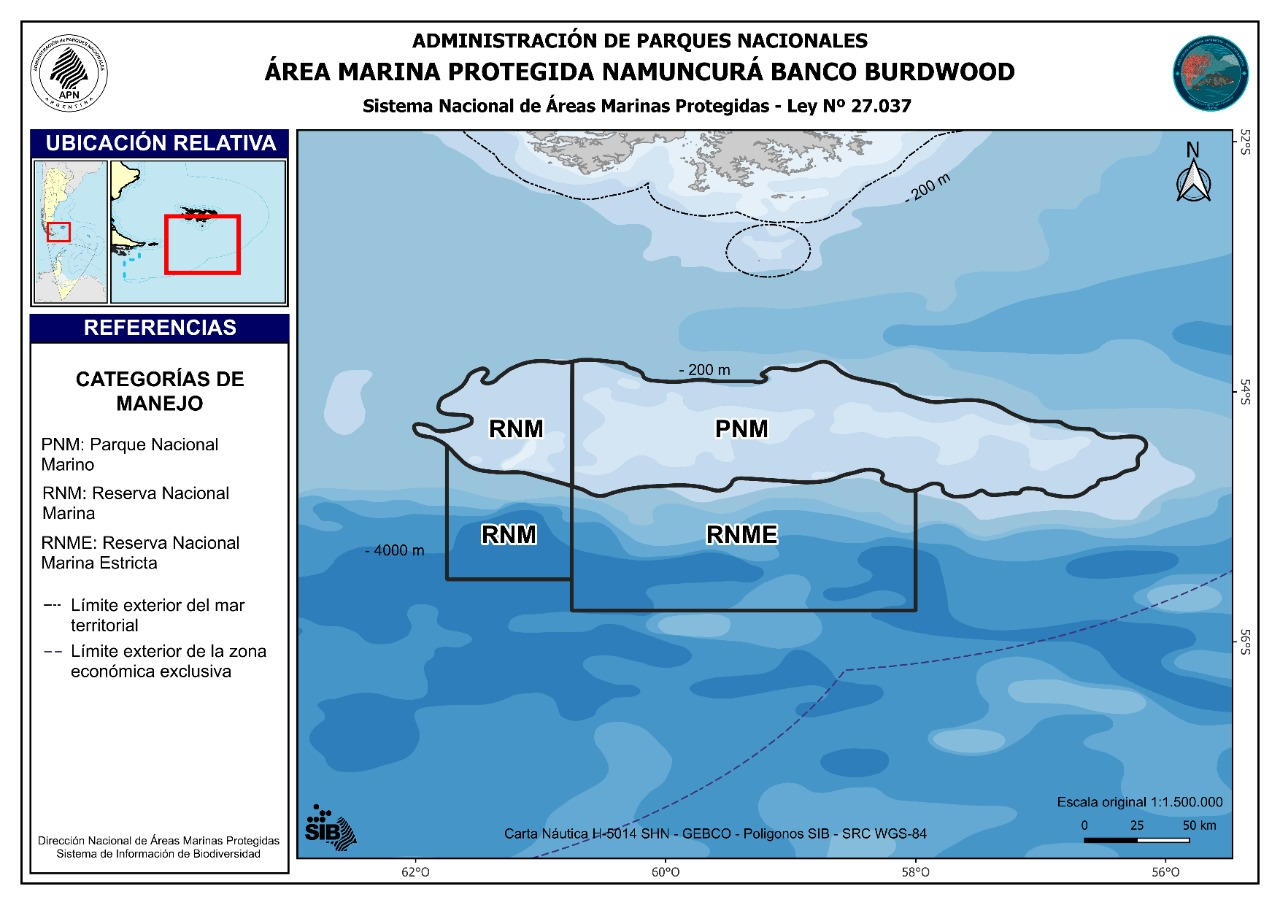
\includegraphics[width=1\linewidth]{MPABurdwood_map} \caption{Map of the Marine Protected Area Namuncurá - Banco Burdwood. Taken from https://www.argentina.gob.ar/parquesnacionales/areasmarinas/namuncura-burdwood.}\label{fig:figure1}
\end{figure}

\hypertarget{network-construction}{%
\subsection{Network construction}\label{network-construction}}

In order to build the network of predator-prey interactions we reviewed
more than 150 references considering published articles, databases and
doctoral theses. Furthermore, we took into account personal
communications from experts belonging to the working group of the study
area (https://www.pampazul.gob.ar/tag/banco-burdwood/). The diversity of
the expertise of the authors contributing to the present study was a key
factor in enhancing the quality of the network, and inherently improved
the network representation of the MPA Namuncurá-Banco Burdwood
ecosystem. A list of the references used to build the network is
presented in Supplementary Material (Table S1).

Due to a lack of trophic data resolution for some species inhabiting the
MPA Namuncurá-Banco Burdwood, we followed the concept of trophic
species, here defined as aggregated groups of taxa. In most cases we
followed this when data on specific biological species were not
available, but for some cases we collapsed species when taxa shared the
same set of predators and prey (trophic similarity criteria). Details
about this can be found in Supplementary Material (Table S2).

With the gathered trophic data we constructed an interaction matrix of
pairwise interactions; a value of 1 or 0 was assigned to each element
a\_ij of the matrix depending on whether the j-species preyed or not on
the i-species. Then we transformed such matrix into an oriented graph
with L trophic interactions between S nodes or species. The orientation
or direction of the graph follows the flow of energy and matter in the
network, from prey to predator.

\hypertarget{network-analysis}{%
\subsection{Network analysis}\label{network-analysis}}

We analysed the MPA Namuncurá - Banco Burdwood network of trophic
interactions, hereafter food web, at two levels: 1) network, considering
species and interactions of the whole network; and 2) species,
considering interactions and species related to a particular species.
The network-level analysis aims to characterize the network of trophic
interactions in terms of complexity and structure. For this we
calculated several network properties commonly used to describe
empirical food webs (Pascual \& Dunne, 2005): (1) number of species S;
(2) number of interactions or links L; (3) link density L/S; (4)
Connectance L/S\^{}2; (5) omnivory Omn; and (6) shortest path length
SPL. Also, we estimated the (7) degree distributions for the food web,
for prey and predators, and for each functional group (e.g.~Amphipoda,
Ascidiacea, Bivalvia, Fish, Marine mammals, Sea birds, etc.) (Table 1).
The prey and predator distributions indicate the frequency of prey among
predators, and viceversa; the functional group's degree shows the
distribution of interactions within groups. The species-level analysis
aims to describe the species' role in the food web. For this we
considered the following properties: (1) betweenness Btw; (2) closeness
Cl; (3) trophic similarity TS; (4) topological role TR; and (5) trophic
level TL (Table 1). We also studied the relationship between species
trophic level and the other species properties by performing linear
regression analyses. Thus, we considered the IS as the dependent
variable and the given unweighted property as the independent variable,
and obtained the coefficients (slope and intercept) for the linear
model. Models were fitted using the least squares approach. We also
explored the mean IS distribution with the species habitat. These
properties provide a general appropriate description of species' role in
empirical complex food webs (Cirtwill et al., 2018).

All network analyses and graphs were performed in R version 4.2.2 (Team,
2022), mainly using `igraph' (Csardi \& Nepusz, 2006) and `multiweb'
(Saravia, 2022) packages. The source code and data are available at
https://github.com/TomasMarina/Banco-Burdwood.

\begin{longtable}[]{@{}
  >{\raggedright\arraybackslash}p{(\columnwidth - 6\tabcolsep) * \real{0.2266}}
  >{\raggedright\arraybackslash}p{(\columnwidth - 6\tabcolsep) * \real{0.2578}}
  >{\raggedright\arraybackslash}p{(\columnwidth - 6\tabcolsep) * \real{0.2578}}
  >{\raggedleft\arraybackslash}p{(\columnwidth - 6\tabcolsep) * \real{0.2578}}@{}}
\caption{List of network and species-level properties analysed,
definitions, and relevant ecological implications related to food web
complexity and structure.}\tabularnewline
\toprule()
\begin{minipage}[b]{\linewidth}\raggedright
\textbf{Name}
\end{minipage} & \begin{minipage}[b]{\linewidth}\raggedright
\textbf{Definition}
\end{minipage} & \begin{minipage}[b]{\linewidth}\raggedright
\textbf{Implications}
\end{minipage} & \begin{minipage}[b]{\linewidth}\raggedleft
\textbf{Reference}
\end{minipage} \\
\midrule()
\endfirsthead
\toprule()
\begin{minipage}[b]{\linewidth}\raggedright
\textbf{Name}
\end{minipage} & \begin{minipage}[b]{\linewidth}\raggedright
\textbf{Definition}
\end{minipage} & \begin{minipage}[b]{\linewidth}\raggedright
\textbf{Implications}
\end{minipage} & \begin{minipage}[b]{\linewidth}\raggedleft
\textbf{Reference}
\end{minipage} \\
\midrule()
\endhead
\textbf{Number of species} & Number of trophic species in a food web. &
It represents the species diversity and has implications for the
persistence of the ecosystem. & May 1973, Tilman 1996 \\
\textbf{Number of interactions} & Total number of trophic interactions
in a food web. & It represents the number of pathways along which matter
and energy can flow. & Dunne et al.~2002 \\
\textbf{Link density} & Ratio of interactions to species in a food web &
It represents the average number of interactions per species; informs
about how connected species are in the food-web. & Dunne et al.~2002 \\
\textbf{Connectance} & Proportion of potential links among species that
are actually realized. & It measures the probability of interactions; it
is a fundamental measure of network complexity. Connectance can be
negatively or positively associated with food web robustness, depending
on the network structure (random vs non-random) or how the strength of
the interactions are distributed. & Martinez 1992 \\
\textbf{Degree distribution} & Frequency of trophic species that have k
or more interactions. & It suggests on the vulnerability of complex food
webs against random failures and intentional attacks (i.e. species
extinctions). & Albert \& Barabási 2002 \\
\textbf{Omnivory} & Species feeding on prey from more than one trophic
level. & It influences food web's stability; intermediate levels of
omnivory may stabilize it and may diffuse top-down effects thus reduce
the probability of trophic cascades. & McCann \& Hastings 1997 \\
\textbf{Shortest path length} & Average shortest path length between all
pairs of species. & A short path length imply a rapid spread of an
impact (e.g.~invasion, population fluctuation, local extinction)
throughout the food web. & Watts \& Strogatz 1998 \\
\textbf{Betweenness} & Number of shortest paths going through a species.
& Species with high betweenness act as ``bridges''; if removed, would
have rapidly spreading effects in the food web. & Freeman 1978, Lai et
al.~2012 \\
\textbf{Closeness} & Number of steps required to reach every other
species from a given species. & The removal of a species with high
closeness will affect the most other species in the food web. & Freeman
1978, Lai et al.~2012 \\
\textbf{Trophic similarity} & Trophic overlap based on shared and unique
resources (prey) and consumers (predators). & It measures one of the
most important aspects of species' niches, the trophic niche, and
functional aspects of biodiversity. & Martinez 1992 \\
\textbf{Topological role} & Species role according to interactions
within and across modules (subgroups of species). & Four roles are
defined: module hub, module specialist, module connector and network
connector. Species with the same role are expected to have similar
topological properties. & Guimera \& Nunes Amaral 2005 \\
\bottomrule()
\end{longtable}

\hypertarget{results}{%
\section{Results}\label{results}}

\hypertarget{network-level-properties}{%
\subsection{Network-level properties}\label{network-level-properties}}

In terms of complexity, the MPA Namuncurá - Banco Burdwood food web
consisted of 1778 predator-prey interactions and 379 species, where 93\%
of them were defined at the species taxonomical level (Figure 2, Table
S2). The food web presented a link density of 4.69, meaning the average
number of interactions per species, and a connectance of 0.01. Almost
half of the consumers were omnivores, feeding on sources at different
trophic levels. The food web showed a path length of 2.99, which implies
that nearly three interactions are needed to connect any pair of species
of the network (Table 1).

\newpage

\begin{figure}

{\centering 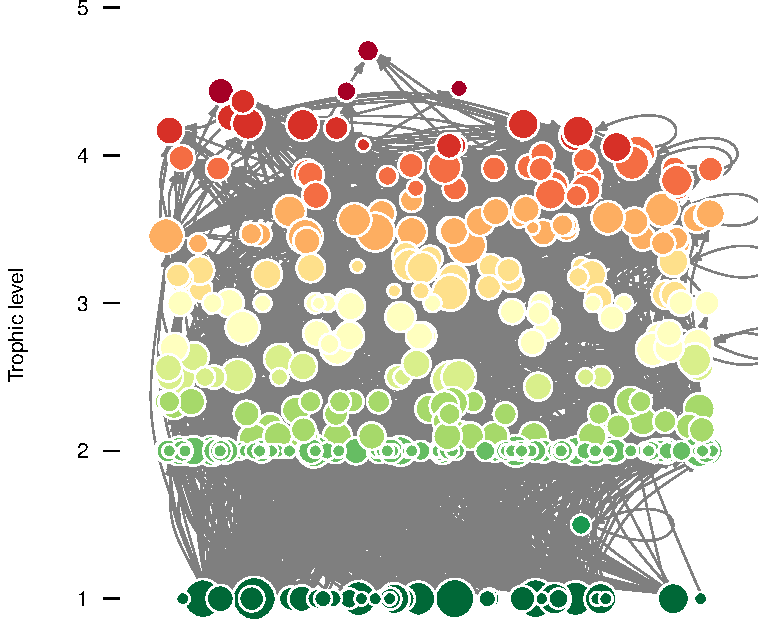
\includegraphics{MS_Burdwood_foodweb_files/figure-latex/figure2-1} 

}

\caption{Graph of the food web for the MPA Namuncurá - Banco Burdwood. Circles represent species and arrows trophic interactions. Circle diameter is relative to the number of interactions. Colour gradient indicate the trophic level.}\label{fig:figure2}
\end{figure}

\begin{table}

\caption{\label{tab:table2}Network-level properties of the MPA Namuncurá - Banco Burdwood food web. See table 1 for definitions and ecological relevance.}
\centering
\begin{tabular}[t]{r|r|r|r|r|r}
\hline
\textbf{Species} & \textbf{Interactions} & \textbf{Density} & \textbf{Connectance} & \textbf{Omnivory} & \textbf{Path length}\\
\hline
379 & 1778 & 4.69 & 0.01 & 0.48 & 2.99\\
\hline
\end{tabular}
\end{table}

The degree distribution of the food web showed an asymmetric frequency
in the number of interactions, where most of the species had a
relatively low number of interactions and few species concentrated the
majority of them (Figure 3A). The distribution of prey among predators
showed that most of the consumers fed on a low number of prey whereas
few of them had multiple preys (Figure 3B). These were the top-five
predators in number of prey: \emph{Patagonotothen guntheri}
(Notothenioid fish, 52 prey), \emph{Patagonotothen ramsayi}
(Notothenioid fish, 50 prey), \emph{Dissostichus eleginoides}
(Notothenioid fish, 30 prey), \emph{Bathyraja brachyurops}
(Chondrichthyan, 30 prey), and \emph{Bathyraja griseocauda}
(Chondrichthyan, 28 prey). Following the same distribution pattern, few
prey presented multiple predators (Figure 3C). These were the top-five
prey in number of predators: Detritus (Non-living, 153 predators), the
three categories of Diatoms considered (benthic, centric and pennate, 72
predators on average), and species of the genus \emph{Euphausia}
(Zooplankton, 46 predators). Finally, taking into account the
interactions within each functional group, again the majority of the
interactions were concentrated in few species (Figure 3D). The most
evident species were: \emph{Themisto gaudichaudii} (Amphipoda),
\emph{Zygochlamys patagonica} (Bivalvia), \emph{Aspidostoma giganteum}
(Bryozoa), \emph{Munida gregaria} (Decapoda), \emph{Patagonotothen
ramsayi} and \emph{Patagonotothen guntheri} (bentho-pelagic fish),
\emph{Psychrolutes marmoratus} (demersal fish), and species of
\emph{Euphausia} (Zooplankton). Overall, there is an evident asymmetry
in the distribution of interactions among species at different levels in
the MPA Namuncurá - Banco Burdwood food web.

A list of the distribution of interactions per species is presented in
Supplementary Material (Table S3).

\begin{figure}

{\centering 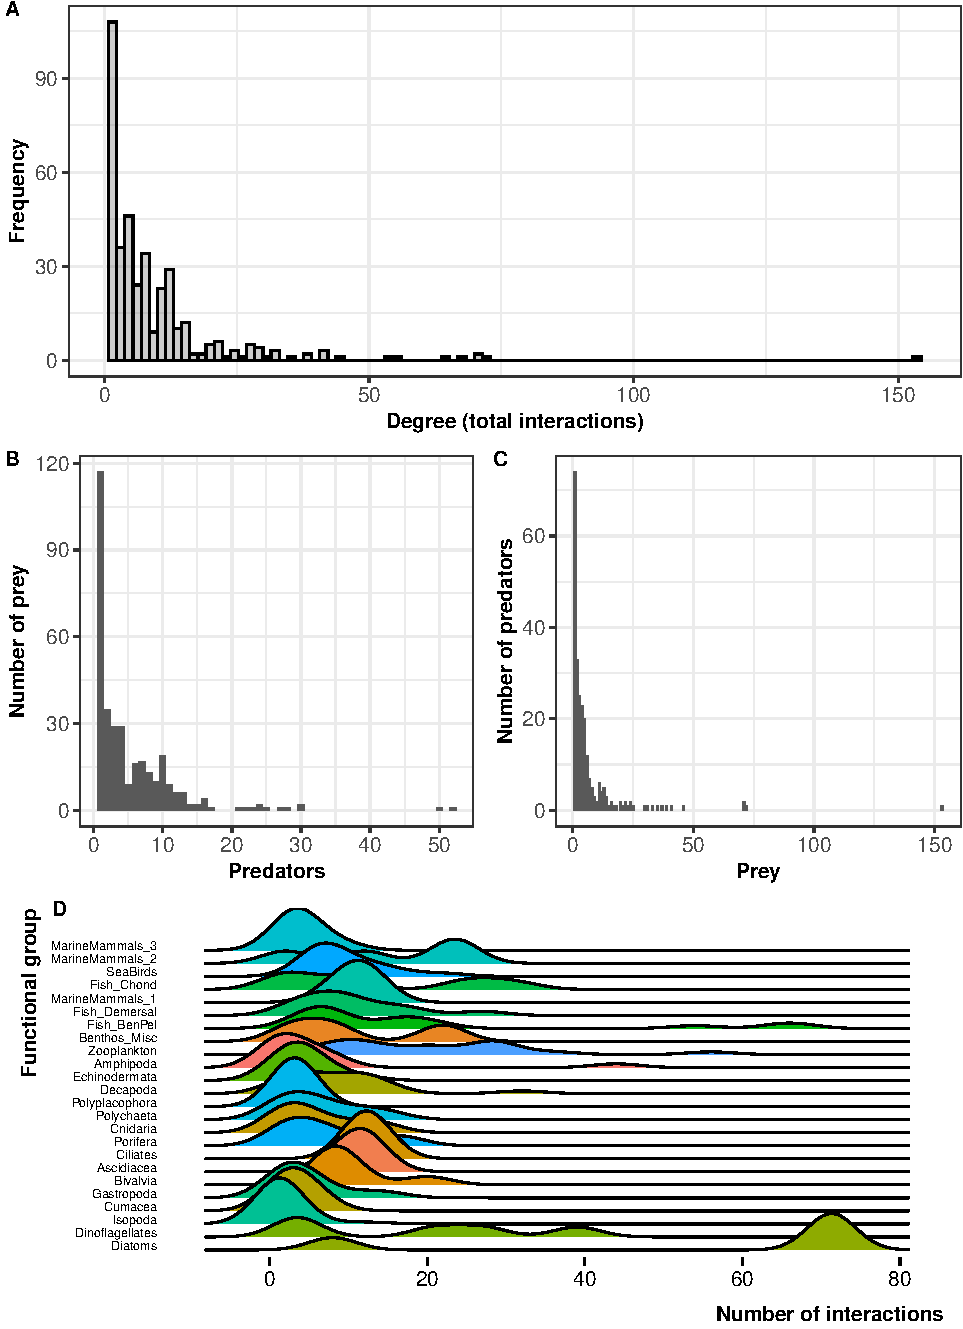
\includegraphics{MS_Burdwood_foodweb_files/figure-latex/figure3-1} 

}

\caption{Degree distributions for the (A) food web, for (B) prey among predators, (C) predators among prey, and (D) for each functional group. Groups are vertically ordered by increasing trophic level; groups with less than 3 species were not plotted (e.g. pelagic fish).}\label{fig:figure3}
\end{figure}

\hypertarget{species-level-properties}{%
\subsection{Species-level properties}\label{species-level-properties}}

The majority of the species of the food web were consumers, 336 out of
379; the rest were primary producers, such as diatoms (phytoplankton),
and non-living food sources like detritus and necromass.

We found different relationships between the species trophic level (TL)
and the rest of the analysed species-level properties (Figure 4A-D). In
this regard, the most evident significant relationship was with trophic
similarity, i.e.~the higher the species' TL, the lower the trophic
similarity or the higher the uniqueness in terms of trophic role (Figure
4C). Here it's noteworthy to highlight high-trophic level species with
low values of trophic similarity: \emph{Bathyraja macloviana} and
\emph{Squalus acanthias} (Chondrichthyans), \emph{Diplopteraster clarki}
and \emph{Pteraster sp} (echinoderms), \emph{Phalacrocorax\_atriceps}
and \emph{Eudyptes chrysocome} (sea birds), and \emph{Lagenorhynchus
cruciger} and \emph{Mesoplodon bowdoini} (marine mammals) (Table S3).

We also found a negative significant relationship with closeness,
however less evident, meaning that low-TL species are relatively closer
to any other species in the food web (Figure 4B). Species of genera
\emph{Calanus} and \emph{Euphausia}, and species of Brachiopoda, all of
them with TL \textless{} 3, registered the highest values of closeness
(Table S3).

It's noteworthy that the highest values of betweenness were shown by
species of mid-TLs (3-4), meaning that those species participated in the
highest number of shortest paths between species (Figure 4A). These were
the species with the highest values: \emph{Patagonotothen ramsayi},
\emph{Dissostichus eleginoides}, \emph{Salilota australis} (fishes),
\emph{Doryteuthis gahi} (Cephalopoda), and \emph{Patagonotothen
guntheri} (Notothenioid fish) (Table S3).

Taking into account the topological role, `module specialist' species
were the most frequent and presented a wide TL range (1 - 4.77); `module
hub' was constrained to mid-TL species (2.48 - 3.92); `module connector'
from low to mid-TLs (1 - 3.86); and `network connector', the least
frequent, had all of its species in TL = 1, except for one with TL =
3.47 (Figure 4D, see Figure S2 for species' topological roles in a food
web graph framework). Here it's important to highlight species of the
two latter topological roles, because they are responsible for linking
modules and maintaining the connectivity of the food web: 40 species (5
network connectors + 35 module connectors) from 20 different functional
groups with a TL range = 1 - 3.86.

An exhaustive list of the species-level properties is presented in
Supplementary Material (Table S3).

\begin{figure}

{\centering 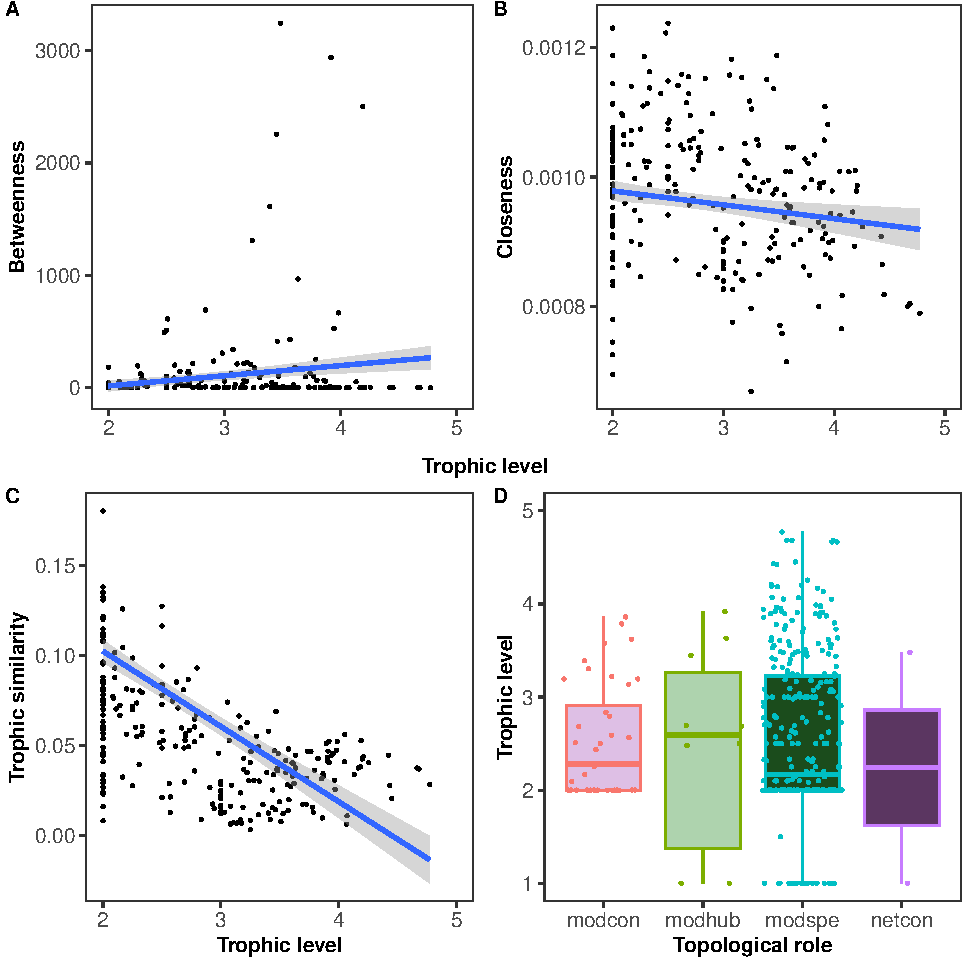
\includegraphics{MS_Burdwood_foodweb_files/figure-latex/figure4-1} 

}

\caption{Species-level properties by trophic level: (A) betweenness, (B) closeness, (C) trophic similarity, and (D) topological role. Each point represents a species. Linear regressions for betweenness ($y = 72.48x - 111.98, R^2 = 0.04, p-value < 3.38e-05$), closeness ($y = 5.78e-06x - 9.37e-04, R^2 = -0.0005, p-value = 0.37$) and trophic similarity ($y = -0.01x - 0.11, R^2 = 0.07, p-value = 6.76e-08$). Note that for A, B and C panels only species with TLs equal or greater than 2 were considered.}\label{fig:figure4}
\end{figure}

\hypertarget{discussion}{%
\section{Discussion}\label{discussion}}

\hypertarget{the-mpa-namuncuruxe1---banco-burdwood-food-web}{%
\subsection{The MPA Namuncurá - Banco Burdwood food
web}\label{the-mpa-namuncuruxe1---banco-burdwood-food-web}}

\begin{itemize}
\item
  The MPA Namuncurá - Banco Burdwood food web is one of the most
  highly-resolved networks of trophic interactions described for
  subpolar and polar regions. Compare network-level properties with
  other subpolar and polar food webs.
\item
  The food web shows an asymmetry in the distribution of interactions at
  several levels: food web, functional group, prey and predators. In all
  of them interactions are concentrated in a few species. On one hand,
  this asymmetry indicates that most consumers have a narrow diet, and
  few present flexible diets (\emph{Patagonotothen guntheri}, \emph{P.
  ramsayi}, \emph{Dissostichus eleginoides}, \emph{Bathyraja
  brachyurops}, \emph{B. griseocauda}). On the other hand few prey are
  consumed by many predators, meaning that there are dominant food
  sources from which most consumers depend on: detritus, diatoms
  (benthic, centric, pennate), and species of \emph{Euphausia}.
\end{itemize}

\hypertarget{species-role}{%
\subsection{Species' role}\label{species-role}}

Our results state that certain species play particular roles in the
structure of the food web.

\begin{itemize}
\item
  Betweenness. Species at mid-trophic levels (3-4) lie in more shortest
  paths between species than any other species: `bridge' role.
  Implications for spread of perturbations like mercury (Fioramonti,
  Ribeiro Guevara, Becker, \& Riccialdelli, 2022), microplastics (Cossi
  et al., 2021).
\item
  Closeness. Low-trophic level species are relatively closer to other
  species in the food web. Apart from the most demanded food sources
  (i.e.~detritus), which are logically closer to many species,
  unexpected consumers arise as important in this regard. Species of the
  zooplankton community like \emph{Calanus} and \emph{Euphausia} are
  crucial for the food web functioning, since they can affect others
  more quickly.
\item
  Trophic similarity. Species are more similar at low and mid-trophic
  levels (2-4). There is a functional redundancy at these levels of the
  food web. On the other hand, less trophic similarity at high TLs
  indicate uniqueness in terms of trophic role. This highlights the
  importance of top predators in the sense that they play a role that
  cannot be played by any other species.
\item
  Topological role. Low and mid-trophic level species (TL = 1 - 3.86)
  are responsible for maintaining the connectivity of the food web
  (network connector and module connector). The functional groups
  represented are: Amphipoda, Bivalvia, Bryozoa, Cnidaria, Cumacea,
  Decapoda, Detritus, Diatoms, Echinodermata, Fish (bentho-pelagic,
  demersal, chondrichthyes), Foraminifera, Polychaeta, Porifera,
  Zooplankton. This shows that the structure of the food web depends on
  a diversity of species, which at the end comprise the ecosystem's
  diversity.
\item
  Overall, low and mid-trophic level species arise as crucial in the
  structure of the MPA Namuncurá - Banco Burdwood food web, since they
  present the highest betweenness and closeness values, and the most
  important topological roles. This coincides with a recent study that
  suggest a wasp-waist trophic structure for the region (Riccialdelli et
  al., 2020). However, we also suggest that there exists functional
  redundancy at mid-trophic levels. Furthermore, our study points out
  species of high-trophic levels due to its uniqueness role.
\end{itemize}

\hypertarget{caveats-and-future-perspectives}{%
\subsection{Caveats and future
perspectives}\label{caveats-and-future-perspectives}}

Caveats:

\begin{itemize}
\item
  Seasonal variation in predators' diet due to food source availability.
\item
  Spatial variation of study area: Banco Burdwood west-east gradient.
\item
  The lack of density or biomass data might have neglected well-known
  important species for the structure of the food web: \emph{Sprattus
  fuegensis}.
\end{itemize}

Perspectives:

\begin{itemize}
\item
  Estimation of interaction strength to gain insights into food web
  stability and response to anthropogenic and environmental
  perturbations.
\item
  Simulate perturbations on food web and target species: mercury
  transfer, microplastic pollution, fisheries.
\end{itemize}

\hypertarget{conclusion}{%
\section{Conclusion}\label{conclusion}}

\hypertarget{references}{%
\section*{References}\label{references}}
\addcontentsline{toc}{section}{References}

\hypertarget{refs}{}
\begin{CSLReferences}{1}{0}
\leavevmode\vadjust pre{\hypertarget{ref-Acha2004}{}}%
Acha, E. M., Mianzan, H. W., Guerrero, R. A., Favero, M., \& Bava, J.
(2004). Marine fronts at the continental shelves of austral {South
America}: {Physical} and ecological processes. \emph{Journal of Marine
Systems}, \emph{44}(1), 83--105. doi:
\href{https://doi.org/10.1016/j.jmarsys.2003.09.005}{10.1016/j.jmarsys.2003.09.005}

\leavevmode\vadjust pre{\hypertarget{ref-Albert2002}{}}%
Albert, R., \& Barabási, A.-L. (2002). Statistical mechanics of complex
networks. \emph{Reviews of Modern Physics}, \emph{74}(1), 47--97. doi:
\href{https://doi.org/10.1103/RevModPhys.74.47}{10.1103/RevModPhys.74.47}

\leavevmode\vadjust pre{\hypertarget{ref-APN2022}{}}%
APN. (2022). \emph{Plan de gestión {AMP Namuncurá Banco Burdwood}}.

\leavevmode\vadjust pre{\hypertarget{ref-Borrelli2014}{}}%
Borrelli, J. J., \& Ginzburg, L. R. (2014). Why there are so few trophic
levels: {Selection} against instability explains the pattern. \emph{Food
Webs}, \emph{1}(1), 10--17. doi:
\href{https://doi.org/10.1016/j.fooweb.2014.11.002}{10.1016/j.fooweb.2014.11.002}

\leavevmode\vadjust pre{\hypertarget{ref-Cirtwill2018}{}}%
Cirtwill, A. R., Dalla Riva, G. V., Gaiarsa, M. P., Bimler, M. D.,
Cagua, E. F., Coux, C., \& Dehling, D. M. (2018). A review of species
role concepts in food webs. \emph{Food Webs}, \emph{16}, e00093. doi:
\href{https://doi.org/10.1016/j.fooweb.2018.e00093}{10.1016/j.fooweb.2018.e00093}

\leavevmode\vadjust pre{\hypertarget{ref-Cossi2021}{}}%
Cossi, P. F., Ojeda, M., Chiesa, I. L., Rimondino, G. N., Fraysse, C.,
Calcagno, J., \& Pérez, A. F. (2021). First evidence of microplastics in
the {Marine Protected Area Namuncurá} at {Burdwood Bank}, {Argentina}: A
study on {Henricia} obesa and {Odontaster} penicillatus
({Echinodermata}: {Asteroidea}). \emph{Polar Biology}, \emph{44}(12),
2277--2287. doi:
\href{https://doi.org/10.1007/s00300-021-02959-5}{10.1007/s00300-021-02959-5}

\leavevmode\vadjust pre{\hypertarget{ref-Csardi2006}{}}%
Csardi, \& Nepusz. (2006). \emph{The igraph software package for complex
network research}.

\leavevmode\vadjust pre{\hypertarget{ref-Dunne2002}{}}%
Dunne, J. A., Williams, R. J., \& Martinez, N. D. (2002). Network
structure and biodiversity loss in food webs: Robustness increases with
connectance. \emph{Ecology Letters}, \emph{5}(4), 558--567. doi:
\href{https://doi.org/10.1046/j.1461-0248.2002.00354.x}{10.1046/j.1461-0248.2002.00354.x}

\leavevmode\vadjust pre{\hypertarget{ref-Fioramonti2022}{}}%
Fioramonti, N. E., Ribeiro Guevara, S., Becker, Y. A., \& Riccialdelli,
L. (2022). Mercury transfer in coastal and oceanic food webs from the
{Southwest Atlantic Ocean}. \emph{Marine Pollution Bulletin},
\emph{175}, 113365. doi:
\href{https://doi.org/10.1016/j.marpolbul.2022.113365}{10.1016/j.marpolbul.2022.113365}

\leavevmode\vadjust pre{\hypertarget{ref-Freeman1978}{}}%
Freeman, L. C. (1978). Centrality in social networks conceptual
clarification. \emph{Social Networks}, \emph{1}(3), 215--239. doi:
\href{https://doi.org/10.1016/0378-8733(78)90021-7}{10.1016/0378-8733(78)90021-7}

\leavevmode\vadjust pre{\hypertarget{ref-Glorioso1995}{}}%
Glorioso, P. D., \& Flather, R. A. (1995). A barotropic model of the
currents off {SE South America}. \emph{Journal of Geophysical Research:
Oceans}, \emph{100}(C7), 13427--13440. doi:
\href{https://doi.org/10.1029/95JC00942}{10.1029/95JC00942}

\leavevmode\vadjust pre{\hypertarget{ref-Guerrero1999}{}}%
Guerrero, R. A., Baldoni, A. G., \& Benavides, H. R. (1999).
\emph{Oceanographic conditions at the southern end of the argentine
continental slope}. doi: \url{http://10.0.64.26/handle/inidep/247}

\leavevmode\vadjust pre{\hypertarget{ref-Guimera2005}{}}%
Guimerà, R., \& Nunes Amaral, L. A. (2005). Functional cartography of
complex metabolic networks. \emph{Nature}, \emph{433}(7028), 895--900.
doi: \href{https://doi.org/10.1038/nature03288}{10.1038/nature03288}

\leavevmode\vadjust pre{\hypertarget{ref-Lai2012}{}}%
Lai, S.-M., Liu, W.-C., \& Jordán, F. (2012). On the centrality and
uniqueness of species from the network perspective. \emph{Biology
Letters}, \emph{8}(4), 570--573. doi:
\href{https://doi.org/10.1098/rsbl.2011.1167}{10.1098/rsbl.2011.1167}

\leavevmode\vadjust pre{\hypertarget{ref-Lopez-Gappa2018}{}}%
López-Gappa, J., Liuzzi, M. G., \& Zelaya, D. G. (2018). A new genus and
species of cheilostome bryozoan associated with hermit crabs in the
subantarctic {Southwest Atlantic}. \emph{Polar Biology}, \emph{41}(4),
733--741. doi:
\href{https://doi.org/10.1007/s00300-017-2234-9}{10.1007/s00300-017-2234-9}

\leavevmode\vadjust pre{\hypertarget{ref-Martinez1992}{}}%
Martinez, N. D. (1992). Constant {Connectance} in {Community Food Webs}.
\emph{The American Naturalist}, \emph{139}(6), 1208--1218. doi:
\href{https://doi.org/10.1086/285382}{10.1086/285382}

\leavevmode\vadjust pre{\hypertarget{ref-Matano2019}{}}%
Matano, R. P., Palma, E. D., \& Combes, V. (2019). The {Burdwood Bank
Circulation}. \emph{Journal of Geophysical Research: Oceans},
\emph{124}(10), 6904--6926. doi:
\href{https://doi.org/10.1029/2019JC015001}{10.1029/2019JC015001}

\leavevmode\vadjust pre{\hypertarget{ref-Matusevich2022}{}}%
Matusevich. (2022). \emph{Chondrichthyan fauna from the {Marine
Protected Area Namuncurá} at {Burdwood Bank}: Exploring egg nursery
grounds}. https://www.researchsquare.com. doi:
\href{https://doi.org/10.21203/rs.3.rs-2247873/v1}{10.21203/rs.3.rs-2247873/v1}

\leavevmode\vadjust pre{\hypertarget{ref-May1973}{}}%
May, R. (1973). \emph{Stability and complexity in model ecosystems}.
{Princeton University Press}.

\leavevmode\vadjust pre{\hypertarget{ref-McCann1997}{}}%
McCann, K., \& Hastings, A. (1997). Re\textendash evaluating the
omnivory\textendash stability relationship in food webs.
\emph{Proceedings of the Royal Society of London. Series B: Biological
Sciences}, \emph{264}(1385), 1249--1254. doi:
\href{https://doi.org/10.1098/rspb.1997.0172}{10.1098/rspb.1997.0172}

\leavevmode\vadjust pre{\hypertarget{ref-Pascual2005}{}}%
Pascual, M., \& Dunne, J. A. (2005). \emph{Ecological {Networks}:
{Linking Structure} to {Dynamics} in {Food Webs}}. {Oxford University
Press}.

\leavevmode\vadjust pre{\hypertarget{ref-Pastorino2019}{}}%
Pastorino, G. (2019). A new deep water gastropod of the genus
{Parabuccinum} ({Neogastropoda}: {Buccinulidae}) from southwestern
{Atlantic} waters with new data on the distribution of all species.
\emph{Marine Biodiversity}, \emph{49}(2), 913--922. doi:
\href{https://doi.org/10.1007/s12526-018-0876-7}{10.1007/s12526-018-0876-7}

\leavevmode\vadjust pre{\hypertarget{ref-Piola1989}{}}%
Piola, A. R., \& Gordon, A. L. (1989). Intermediate waters in the
southwest {South Atlantic}. \emph{Deep Sea Research Part A.
Oceanographic Research Papers}, \emph{36}(1), 1--16. doi:
\href{https://doi.org/10.1016/0198-0149(89)90015-0}{10.1016/0198-0149(89)90015-0}

\leavevmode\vadjust pre{\hypertarget{ref-Piola2009}{}}%
Piola, A., \& Falabella, V. (2009). \emph{El mar {Patagónico}}.
{Wildlife Conservation Society y Birdlife Internacional}.

\leavevmode\vadjust pre{\hypertarget{ref-Reta2014}{}}%
Reta, R. (2014). \emph{Oceanografía del {Banco Burdwood}: {Estado
Actual} del {Conocimiento} y {Perspectivas}}. {INIDEP}.

\leavevmode\vadjust pre{\hypertarget{ref-Riccialdelli2020}{}}%
Riccialdelli, L., Becker, Y. A., Fioramonti, N. E., Torres, M., Bruno,
D. O., Rey, A. R., \& Fernández, D. A. (2020). Trophic structure of
southern marine ecosystems: A comparative isotopic analysis from the
{Beagle Channel} to the oceanic {Burdwood Bank} area under a wasp-waist
assumption. \emph{Marine Ecology Progress Series}, \emph{655}, 1--27.
doi: \href{https://doi.org/10.3354/meps13524}{10.3354/meps13524}

\leavevmode\vadjust pre{\hypertarget{ref-Saravia2022a}{}}%
Saravia, L. A. (2022). \emph{Multiweb: {Ecological} network analyses
including multiplex networks}.

\leavevmode\vadjust pre{\hypertarget{ref-Schejter2016}{}}%
Schejter, L., Rimondino, C., Chiesa, I., Díaz de Astarloa, J. M., Doti,
B., Elías, R., \ldots{} Bremec, C. S. (2016). Namuncurá {Marine
Protected Area}: An oceanic hot spot of benthic biodiversity at
{Burdwood Bank}, {Argentina}. \emph{Polar Biology}, \emph{39}(12),
2373--2386. doi:
\href{https://doi.org/10.1007/s00300-016-1913-2}{10.1007/s00300-016-1913-2}

\leavevmode\vadjust pre{\hypertarget{ref-RCoreTeam2022}{}}%
Team, R. C. (2022). \emph{R: {A Language} and {Environment} for
{Statistical Computing}}. {Vienna, Austria}: R Foundation for
Statistical Computing.

\leavevmode\vadjust pre{\hypertarget{ref-Tilman1996}{}}%
Tilman, D. (1996). Biodiversity: {Population Versus Ecosystem
Stability}. \emph{Ecology}, \emph{77}(2), 350--363. doi:
\href{https://doi.org/10.2307/2265614}{10.2307/2265614}

\leavevmode\vadjust pre{\hypertarget{ref-Watts1998}{}}%
Watts, D. J., \& Strogatz, S. H. (1998). Collective dynamics of
{``small-world''} networks. \emph{Nature}, \emph{393}(6684), 440--442.
doi: \href{https://doi.org/10.1038/30918}{10.1038/30918}

\end{CSLReferences}


\end{document}
